\section{Git workflow}

\subsection{The main branches}

At the core, the development model is greatly inspired by existing models out
there. The central repo holds two main branches with an infinite lifetime:
\begin{itemize}[itemsep=1pt, parsep=1pt]
  \item master
  \item development
\end{itemize}

We consider origin/master to be the main branch where the source code of HEAD
always reflects a production-ready state.We consider origin/develop to be the
main branch where the source code of HEAD always reflects a state with the latest
delivered development changes for the next release. Some would call this the
“integration branch”.

When the source code in the develop branch reaches a stable point and is ready to
be released, all of the changes should be merged back into master somehow and
then tagged with a release number.Therefore, each time when changes are merged
back into master, this is a new production release by definition. For the first
weeks we have ignored all this workflow and worked directly on the master
branch, but since we are documenting the workflow process we agreed that's
better to revert to some solid guidelines and use Git to its full
potential.\footnote{The tag point identifying this radical change is name
\textbf{end\_of\_anarchy}}

\subsection{Supporting branches}

Next to the main branches master and development, our development model uses a
variety of supporting branches to aid parallel development between team members,
ease tracking of features, prepare for production releases and to assist in
quickly fixing live production problems. Unlike the main branches, these branches
always have a limited life time, since they will be removed eventually. The
different types of branches we may use are: \begin{itemize}[itemsep=1pt,
parsep=1pt]
  \item Release
  \item Hotfix
  \item Testing
  \item Report
\end{itemize}

Each of these branches have a specific purpose and are bound to strict rules as
to which branches may be their originating branch and which branches must be
their merge targets.By no means are these branches “special” from a technical
perspective. The branch types are categorized by how we use them.

\begin{figure}[!htb]
  \begin{center}
    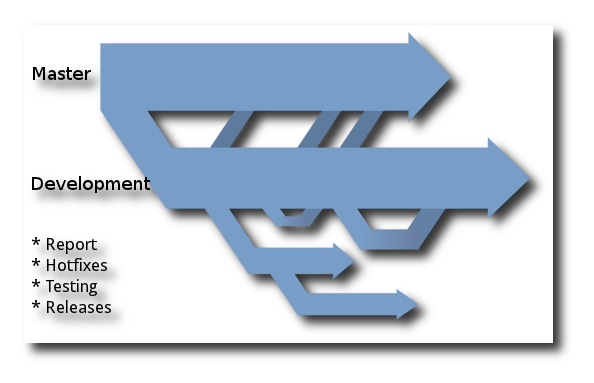
\includegraphics{Figures/Branches.eps}
  \end{center}
  \label{Git repository branches}
  \caption{Git repository branches}
\end{figure}

\subsection{Report branche}
This branch is quite unique in the project because it's where the project report
is writeen. Being a \LaTeX project it is not bended by the general
development rules, beside the fact that we have one person doing the reporting
part and the other reviewing it. For these raison, and because we have the
obligation to provide the supervisor with pdf file and we don't enjoy the
thaught of having many binary files in the repository we decided to adopt a
pragmatic management model:
\begin{enumerate}
  \item All the development in the report are added by all developers but
  compiled and not commited in the local repositories.
  \item When a certain amount of changes are judged significant enough, the
  report is compiled to produce the pdf file which will be then commited to the
  repository.
  \item Only when pdf file is validated by both developpers and suppervisor, the
  branch is merge in the release and then in master branch.
\end{enumerate}

Because of the implication of this model, the Report branch is unique and not
removed from the repository.

\subsubsection{Testing branches}
\begin{itemize}
  \item May branch off from: developement
  \item Must merge back into: development and master
  \item Branch naming convention: testing-*
\end{itemize}
Testing branches are the final validation of the features development.
\todo[size=\footnotesize]{Describe the testing model used JUnit or Code coverage
and the implication on code}

\subsubsection{Release branches}
\begin{itemize}[itemsep=1pt, parsep=1pt]
  \item May branch off from: development
  \item Must merge back into: development and master
  \item Branch naming convention: release-* 
\end{itemize}

Release branches support preparation of a new production release. Furthermore,
they allow for minor bug fixes and preparing meta-data for a release (version
number, build dates, etc.). By doing all of this work on a release branch, the
develop branch is cleared to receive features for the next big release.

The key moment to branch off a new release branch from develop is when develop
(almost) reflects the desired state of the new release. At least all features
that are targeted for the release-to-be-built must be merged in to develop at
this point in time. All features targeted at future releases may not—they must
wait until after the release branch is branched off.

It is exactly at the start of a release branch that the upcoming release gets
assigned a version number—not any earlier. Up until that moment, the develop
branch reflected changes for the “next release”, but it is unclear whether that
“next release” will eventually become 0.3 or 1.0, until the release branch is
started.

\paragraph{Creating a release branch}
Release branches are created from the develop branch. For example, say version
1.1.5 is the current production release and we have a big release coming up. The
state of develop is ready for the “next release” and we have decided that this
will become version 1.2. So we branch off and give the release branch a name
reflecting the new version number:
\begin{verbatim}
$ git checkout -b release-1.2 development
Switched to a new branch "release-1.2"
$ git commit -a -m "Bumped version number to 1.2"
[release-1.2 74d9424] Bumped version number to 1.2
1 files changed, 1 insertions(+), 1 deletions(-)
\end{verbatim}

This new branch may exist there for a while, until the release may be rolled out
definitely. During that time, bug fixes may be applied in this branch (rather
than on the develop branch). Adding large new features here is strictly
prohibited. They must be merged into develop, and therefore, wait for the next
big release. Finishing a release branch

When the state of the release branch is ready to become a real release, some
actions need to be carried out. First, the release branch is merged into master .
Next, that commit on master must be tagged for easy future reference to this
historical version. Finally, the changes made on the release branch need to be
merged back into development, so that future releases also contain these bug
fixes. The first two steps in Git:
\begin{verbatim}
$ git checkout master
Switched to branch 'master'
$ git merge --no-ff release-1.2
Merge made by recursive.
(Summary of changes)
$ git tag -a 1.2
\end{verbatim}

The release is now done, and tagged for future reference. To keep the changes
made in the release branch, we need to merge those back into develop, though. In Git:
\begin{verbatim}
$ git checkout development
Switched to branch 'development'
$ git merge --no-ff release-1.2
Merge made by recursive.
(Summary of changes)
\end{verbatim}

Now we are really done and the release branch may be removed, since we don’t
need it anymore:
\begin{verbatim}
$ git branch -d release-1.2
Deleted branch release-1.2 (was ff452fe).
\end{verbatim}

\subsubsection{Hotfix branches}
\begin{itemize}[itemsep=1pt, parsep=1pt]
  \item May branch off from: master
  \item Must merge back into: development and master
  \item Branch naming convention: hotfix-* 
\end{itemize}

Hotfix branches are very much like release branches in that they are also meant
to prepare for a new production release, albeit unplanned. They arise from the
necessity to act immediately upon an undesired state of a live production
version. When a critical bug in a production version must be resolved
immediately, a hotfix branch may be branched off from the corresponding tag on
the master branch that marks the production version.

The essence is that work of team members (on the develop branch) can continue,
while another person is preparing a quick production fix. Creating the hotfix
branch

Hotfix branches are created from the master branch. For example, say version 1.2
is the current production release running live and causing troubles due to a
severe bug. But changes on develop are yet unstable. We may then branch off a
hotfix branch and start fixing the problem:
\begin{verbatim}
$ git checkout -b hotfix-1.2.1 master
Switched to a new branch "hotfix-1.2.1"
$ git commit -a -m "Bumped version number to 1.2.1"
[hotfix-1.2.1 41e61bb] Bumped version number to 1.2.1
1 files changed, 1 insertions(+), 1 deletions(-)
\end{verbatim}
Then, fix the bug and commit the fix in one or more separate commits.
\begin{verbatim}
$ git commit -m "Fixed severe production problem"
[hotfix-1.2.1 abbe5d6] Fixed severe production problem
5 files changed, 32 insertions(+), 17 deletions(-)
\end{verbatim}

\subsubsection{Finishing a hotfix branch}

When finished, the bugfix needs to be merged back into master, but also needs to
be merged back into development, in order to safeguard that the bugfix is
included in the next release as well. This is completely similar to how release
branches are finished. First, update master and tag the release.
\begin{verbatim}
$ git checkout master
Switched to branch 'master'
$ git merge --no-ff hotfix-1.2.1
Merge made by recursive.
(Summary of changes)
$ git tag -a 1.2.1
\end{verbatim}

Next, include the bugfix in development, too:

\begin{verbatim}
$ git checkout development
Switched to branch 'development'
$ git merge --no-ff hotfix-1.2.1
Merge made by recursive.
(Summary of changes)
\end{verbatim}

Finally, remove the temporary branch:
\begin{verbatim}
$ git branch -d hotfix-1.2.1
Deleted branch hotfix-1.2.1 (was abbe5d6).
\end{verbatim}
